\chapter{Arhitektura i dizajn sustava}
		\texttt{}{ Arhitekturu projektnog sustava možemo podijeliti u 3 cjeline:}
	\begin{itemize}
		\item 	\textit{Web aplikacija }
		\item 	\textit{Web poslužitelj}
		\item 	\textit{Baza podataka }		
	\end{itemize}


                \texttt{}{
             Web preglednik je dio arhitekture koji korisniku omogućuje pregled web stranice i svih sadržaja na njoj. Svaki internetski preglednik je prevoditelj. Korisnik putem web preglednika šalje zahtjev web poslužitelju. 
            }

            
                \texttt{}{
             Web poslužitelj osnova je rada web aplikacije. Njegov primaran zadatak je komunikacija klijenta s aplikacijom. Komunikacija se odvija preko HTTP (engl. Hyper Text Transfer Protocol) protokola, sto je protokol u prijenosu informacija na webu. Poslužitelj je onaj koji pokreće web aplikaciju te joj prosljeđuje zahtjev
            }


            
                \texttt{}{
            Korisnik koristi web aplikaciju za obrađivanje željenih zahtijeva. Web aplikacija obrađuje zahtjev te ovisno o zahtjevu, pristupa bazi podataka nakon čega preko poslužitelja vraća korisniku odgovor u obliku HTML dokumenta vidljivog u web pregledniku.}
               

                \texttt{}{
             Null grupa 2022./2023. za projekt na predmetu Programsko inženjerstvo 2022./2023. odabrala je Angular sustav za izradu frontenda (dijela sustava vidljivoga korisniku) i Express sustav za izradu backenda (dijela sustava koji nije vidljiv korisniku) projetknog zadatka. 
            Arhitektura AngularJS-a temelji se na MVC dizajnu (Model, view, controller).
            Model View Controller ili MVC kako se popularno naziva, uzorak je dizajna softvera za razvoj web aplikacija. MVC dizajn sastoji se od sljedeća tri dijela:
            }
            \begin{itemize}
		\item 	\text{ Model je najniža razina uzorka odgovornog za održavanje podataka. }
		\item 	\text{ Prikaz(view) odgovoran je za prikazivanje svih ili dijela podataka korisniku.}
		\item 	\text{Kontroler je softverski kod koji kontrolira interakcije između modela i prikaza.}		
	\end{itemize}
        \eject

             \begin{figure}[H]
			            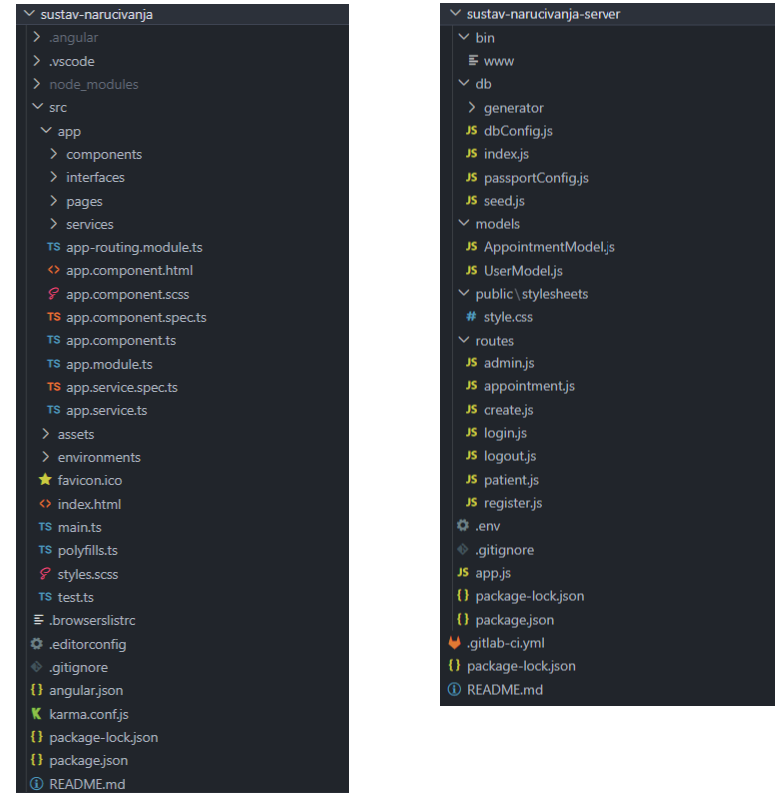
\includegraphics[width=\textwidth]{slike/struktura.png} %veličina u odnosu na širinu linije
			            \caption{Struktura implementacije aplikacije iz VSC.}
			            \label{fig:struktura} %label mora biti drugaciji za svaku sliku
		            \end{figure}

              
               \texttt{}{ Aplikaciju smo rastavili na komponente, sučelja, stranice i servise. 
               Komponente su implementirani dijelovi stranice koje možemo ubaciti kao cjelinu u neku od pages(stranica) kako ne bismo morali pisati dupli kod. Pages(stranice) su sve stranice u našoj aplikaciji. Svaki "page" sastavljen je od '.html' datoteke za strukturu, '.scss' datoteke za dizajn, '.module.ts' u kojoj možemo Typescriptom napraviti uvoz pojedinog modula Angulara u stranicu i '.ts' u kojoj definiramo putanje i povezivanje svih dokumenata.
               
               }

                \texttt{}{ Backend dio aplikacije izveden je u objektno orijentiranoj paradigmi. Pacijenti, doktori, medicinski tehničari te administratori su predstavljeni objektima koji nasljeđuju od zajedničkog roditelja, klase korisnik. Sve podklase klase korisnik znaju provjeriti svoju lozinku i korisničko ime, spremiti se u bazu te druge detalje koji su vezani za pojedinu klasu. Grupe i pregledi također su izvedeni kao klase koje sadrže metode za spremanje i dohvaćanje iz baze podataka.
               }
        
               \texttt{}{
               Razvojno okruženje koje koristite programeri Null grupe jr Visual Studio Code. Za izradu i doradu koda programeri koriste GitLab sustav.
            Za razvoj dokumentacije grupa će koristiti Overleaf aplikaciju radi sistematičnosti izrade.
               }
            
               %\includegraphics[width=\textwidth{slike/mvc.jpeg}
               
		\section{Baza podataka}
			
		
			
		{PostgresSQL baza podataka sastoji se od 7 tablica. Entitet users je supertip koji se disjointed grana na četiri tablice: admin, patient, doctor i nurse. Primarni ključ svih tih entiteta je id koji se u tablici user automatski generira. Tablica patient također sadrži strani ključ doctorid, jer je pacijent pri registraciji obavezan izabrati svog liječnika. Tablica nurse ima strani ključ teamid, referencu na tablicu team. Također ta vrijednost može biti null jer tehničar ne mora nužno biti dio tima. Isto vrijedi i za liječnika. Uz to on još ima atribut appointmentRule u kojem se sadrži njegovo pravilo o rezervaciji termina. Osim tih tablica također baza podataka sadrži već prije spomenutu tablicu team te appointment. Primarni ključ teama je teamid, a tablica team također sadrži ime tima pod nazivom varijable name. Tablica appointment sadrži primarni ključ appointmentId koji se automatski generira te tri strana ključa. Patientid koji obavezno nije null, referenca na pacijenta koji dolazi na pregled. Druga dva strana ključa doctorId i nurseId su međusobno isključivi, odnosno ako jedan ima vrijednost, drugi mora biti null, jer pacijent dolazi na pregled ili kod liječnika ili kod tehničara. Pregled je također određen timestampom time, vremenom kad je ugovoren i intervalom duration.}
		
			\subsection{Opis tablica}
			

				%\textit{Svaku tablicu je potrebno opisati po zadanom predlošku. Lijevo se nalazi točno ime varijable u bazi podataka, u sredini se nalazi tip podataka, a desno se nalazi opis varijable. Svjetlozelenom bojom označite primarni ključ. Svjetlo plavom označite strani ključ}
				
				
				\begin{longtblr}[
					label=none,
					entry=none
					]{
						width = \textwidth,
						colspec={|X[6,l]|X[6, l]|X[20, l]|}, 
						rowhead = 1,
					} %definicija širine tablice, širine stupaca, poravnanje i broja redaka naslova tablice
					\hline \multicolumn{3}{|c|}{\textbf{users}}	 \\ \hline[3pt]
					\SetCell{LightGreen} id     &   INT     &  	Jedinstveni id svakog korisnika, generira se automatski, primarni ključ tablice korisnik \\ \hline
					name	& VARCHAR &   Ime korisnika	\\ \hline 
					surname & VARCHAR &  Prezime korisnika \\ \hline 
					 phoneNumber & VARCHAR	&  	Telefonski broj korisnika, jedinstven ta svakog korisnika	\\ \hline 
					 mail & VARCHAR	&  	Adresa elektroničke pošte korisnika, jedinstvena za svakog korisnika	\\ \hline 
					password & VARCHAR	&  	Lozinka korisnika za prijavu u sustav	\\ \hline 
					sex & VARCHAR	&  	spol korisnika	\\ \hline 
					dateOdBirth & DATE	&  	Datum rođenja korisnika	\\ \hline 
				\end{longtblr}
				
				\begin{longtblr}[
					label=none,
					entry=none
					]{
						width = \textwidth,
						colspec={|X[6,l]|X[6, l]|X[20, l]|}, 
						rowhead = 1,
					} %definicija širine tablice, širine stupaca, poravnanje i broja redaka naslova tablice
					\hline \multicolumn{3}{|c|}{\textbf{admin}}	 \\ \hline[3pt]
					\SetCell{LightGreen} id     &   INT     &  	Strani ključ, referenca na id u tablici users \\ \hline
				\end{longtblr}
				
			\begin{longtblr}[
					label=none,
					entry=none
					]{
						width = \textwidth,
						colspec={|X[12,l]|X[6, l]|X[20, l]|}, 
						rowhead = 1,
					} %definicija širine tablice, širine stupaca, poravnanje i broja redaka naslova tablice
					\hline \multicolumn{3}{|c|}{\textbf{patient}}	 \\ 
                    \hline[3pt]
					\SetCell{LightGreen} id     &   INT     &  	Strani ključ, referenca na id u tablici users \\ \hline
					\SetCell{LightBlue} doctorid & INT & ID doktora kojeg je pacijent izabrao pri registraciji \\ \hline
                  
					nFailedAppointments   &   INT & Broj ugovorenih pregleda koje je pacjent propustio \\ \hline
                
					notificationMethod   &   VARCHAR & Način na koji će pacijent biti obavješten o pregledima. \\ \hline
				\end{longtblr}
			
			
			\begin{longtblr}[
					label=none,
					entry=none
					]{
						width = \textwidth,
						colspec={|X[6,l]|X[6, l]|X[20, l]|}, 
						rowhead = 1,
					} %definicija širine tablice, širine stupaca, poravnanje i broja redaka naslova tablice
					\hline \multicolumn{3}{|c|}{\textbf{doctor}}	 \\ \hline[3pt]
					\SetCell{LightGreen} id      &   INT     &  	Strani ključ, referenca na id u tablici users \\ \hline
					\SetCell{LightBlue}teamid & INT & Id tima kojem je doktor dodjeljen, može biti null \\\hline
                    \SetCell{} appRule & INT & Pravilo koliko je sati unaprijed pacijent obavezan rezervirati termin. 
                    \\ \hline
				\end{longtblr}
			
			\begin{longtblr}[
					label=none,
					entry=none
					]{
						width = \textwidth,
						colspec={|X[6,l]|X[6, l]|X[20, l]|}, 
						rowhead = 1,
					} %definicija širine tablice, širine stupaca, poravnanje i broja redaka naslova tablice
					\hline \multicolumn{3}{|c|}{\textbf{nurse}}	 \\ \hline[3pt]
					\SetCell{LightGreen} id     &   INT     &  	Strani ključ, referenca na id u tablici users \\ \hline
					\SetCell{LightBlue}teamid & INT & Id tima kojem je medicinska sestra dodjeljena, može biti null \\\hline
				\end{longtblr}
				
				\begin{longtblr}[
					label=none,
					entry=none
					]{
						width = \textwidth,
						colspec={|X[6,l]|X[6, l]|X[20, l]|}, 
						rowhead = 1,
					} %definicija širine tablice, širine stupaca, poravnanje i broja redaka naslova tablice
					\hline \multicolumn{3}{|c|}{\textbf{team}}	 \\ \hline[3pt]
					\SetCell{LightGreen} teamid      &   teamid     &  	Id tima \\ \hline
                    name & VARCHAR & Ime tima \\ \hline
				\end{longtblr}
			
			\begin{longtblr}[
					label=none,
					entry=none
					]{
						width = \textwidth,
						colspec={|X[10,l]|X[6, l]|X[20, l]|}, 
						rowhead = 1,
					} %definicija širine tablice, širine stupaca, poravnanje i broja redaka naslova tablice
					\hline \multicolumn{3}{|c|}{\textbf{appointment}}	 \\ \hline[3pt]
					\SetCell{LightGreen} id       &   INT     &  	Jedinstveni ID pregleda, generira se automatski \\ \hline
					\SetCell{LightBlue}patientid & INT & Strani ključ, ID pacijenta koji je zakazao pregled, ne može biti null \\\hline
					\SetCell{LightBlue}doctorid & INT & Strani ključ, ID doktora koji koji vrši pregled\\\hline
					\SetCell{LightBlue}nurseid & INT & Strani ključ, ID medicinskog tehničara koji vrši pregled \\\hline
					time & TIMESTAMP & Vrijeme u koje je pregled ugovoren \\ \hline
					duration & INTERVAL & Trajanje pregleda \\ \hline
                    created_on & TIMESTAMP & Vrijeme ugovaranja pregleda. \\ \hline
                    changes_from & TIMESTAMP & Vrijeme promjene pregleda.
                    type & VARCHAR & Vrsta pregleda.
                    patient_came & BOOLEAN & Zabilježavanje dolaska pacijenta.
				\end{longtblr}
			
			
			\subsection{Dijagram baze podataka}
				\begin{figure}[H]
			            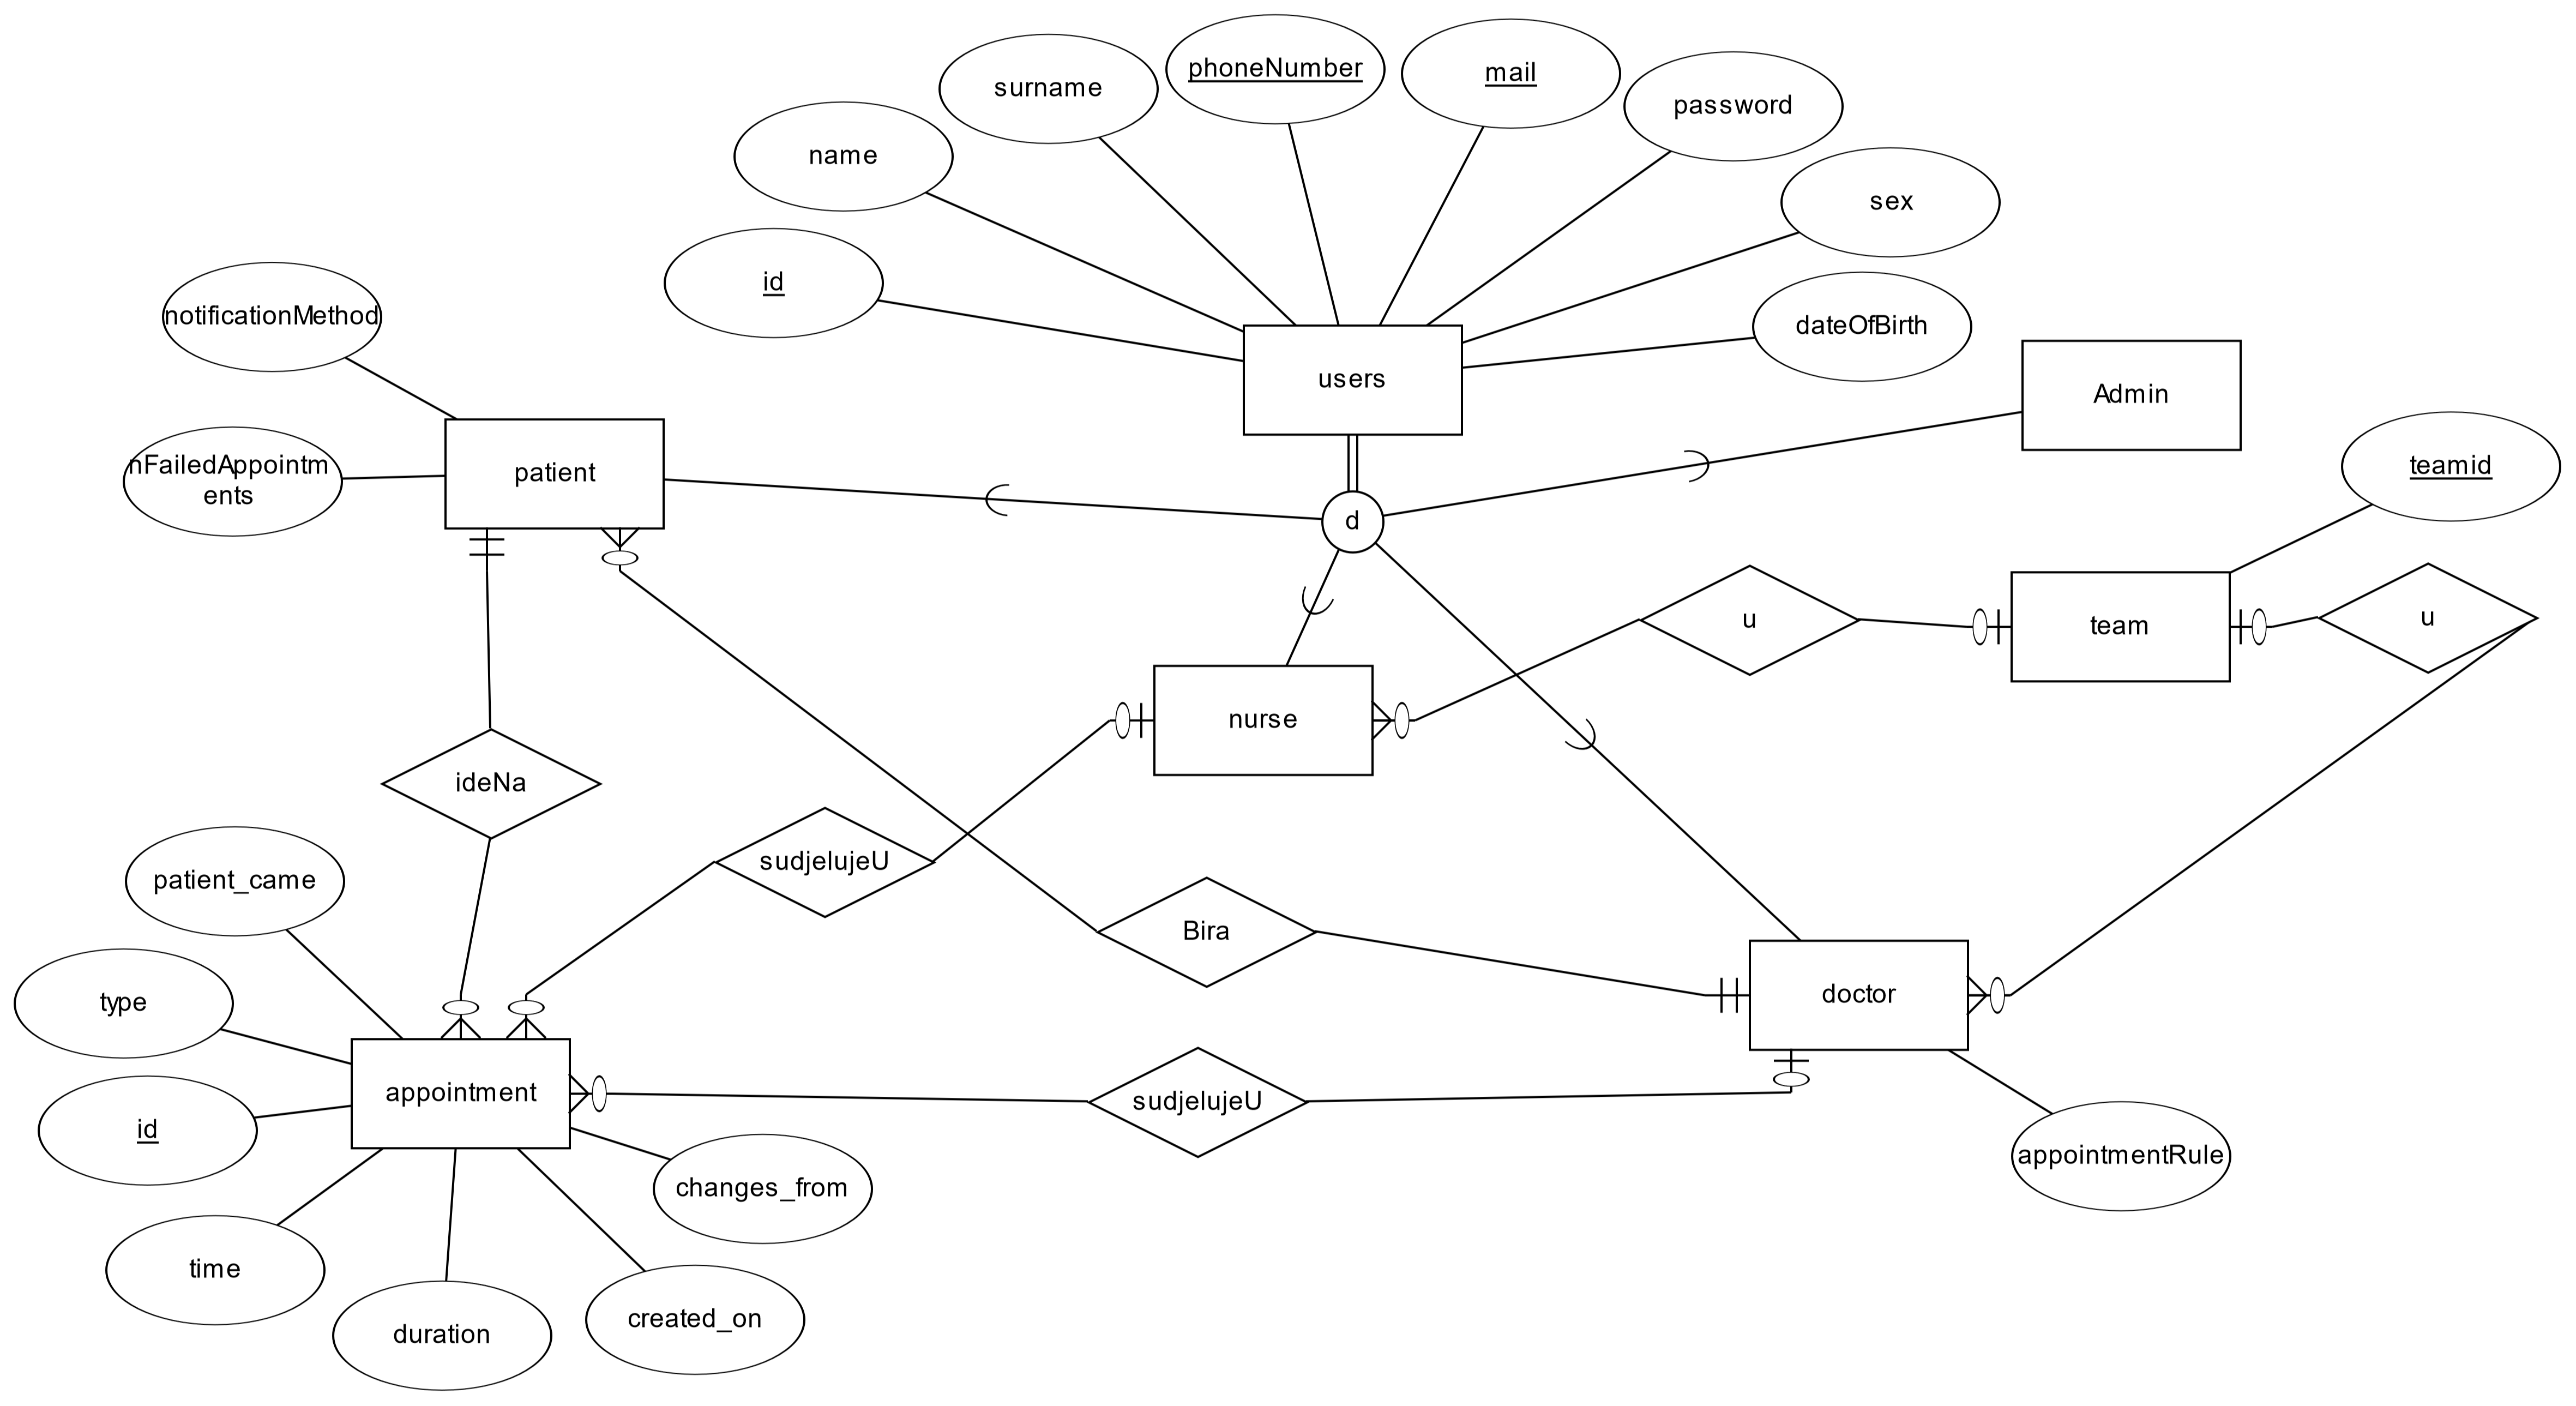
\includegraphics[width=\textwidth]{image.png} %veličina u odnosu na širinu linije
			            \caption{ER dijagram baze podataka}
			            \label{fig:bp1} %label mora biti drugaciji za svaku sliku
		            \end{figure}			
			\subsection{Dijagram baze podataka}
				\begin{figure}[H]
			            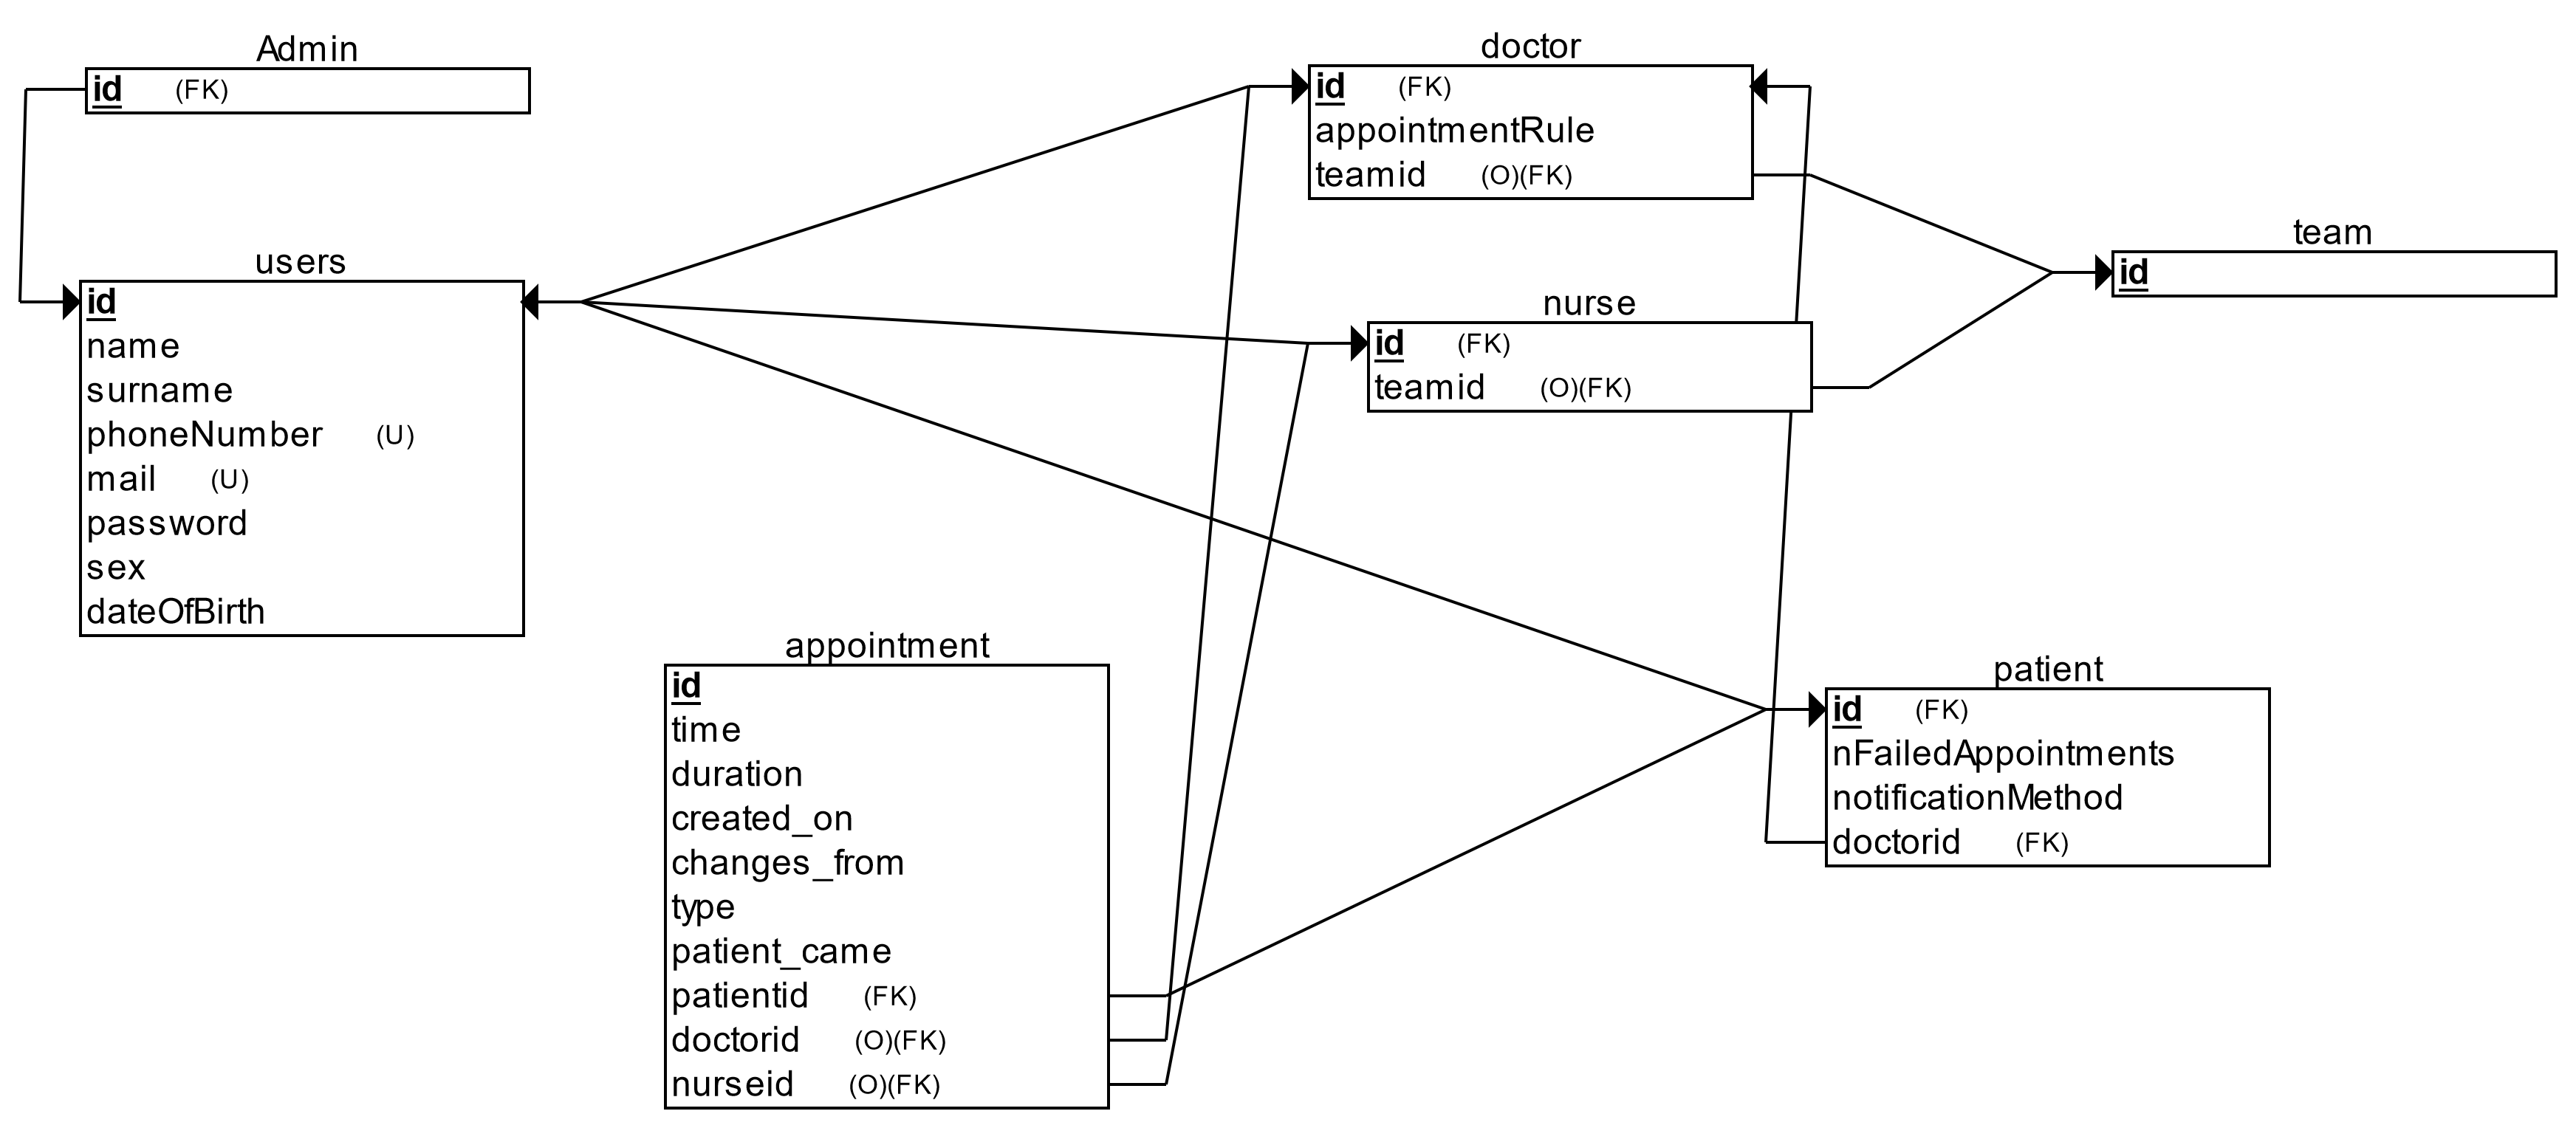
\includegraphics[width=\textwidth]{image(1).png} %veličina u odnosu na širinu linije
			            \caption{Relacijski dijagram baze podataka}
			            \label{fig:bp2} %label mora biti drugaciji za svaku sliku
		            \end{figure}
		            
			
			\eject
			
			
		\section{Dijagram razreda}
		
			%\textit{Potrebno je priložiti dijagram razreda s pripadajućim opisom. Zbog preglednosti je moguće dijagram razlomiti na više njih, ali moraju biti grupirani prema sličnim razinama apstrakcije i srodnim funkcionalnostima.}\\
			
			%\textbf{\textit{dio 1. revizije}}\\
			
			%\textit{Prilikom prve predaje projekta, potrebno je priložiti potpuno razrađen dijagram razreda vezan uz \textbf{generičku funkcionalnost} sustava. Ostale funkcionalnosti trebaju biti idejno razrađene u dijagramu sa sljedećim komponentama: nazivi razreda, nazivi metoda i vrste pristupa metodama (npr. javni, zaštićeni), nazivi atributa razreda, veze i odnosi između razreda.}\\
			
			Na slici 4.4 prikazan je dijagram razreda koji pripada backend dijelu arhitekture. Razredi iz dijagrama predstavljaju strukturu baze podataka u aplikaciji te svaki razred predstavlja jedan entitet iz baze. Metode koje su implementirane komuniciraju s bazom podataka, ako je potrebno, upisuju odgovarajuće podatke u bazu ili ih vraćaju iz baze. Razred User predstavlja svakog korisnika aplikacije i koji može koristiti određene funkcionalnosti sustava. Međutim, prije toga se mora registrirati s osobnim podacima: ime, prezime, spol, broj telefona, e-mail, lozinka i datum rođenja. Razred Pacijent predstavlja korisnika koji je registriran kao pacijent i ima pristup svojim terminima uz funkcionalnosti zakazivanja i otkazivanja termina, kojeg predstavlja razred Appointment. Nešto veću ovlast ima medicinska sestra koju predstavlja razred Nurse, ona može i unaprijed definirati termine usluga. Razred Doctor predstavlja liječnika koji može definirati slobodne termine pregleda, ali i definirati pravila za naručivanje. Najvišu ovlast ima administrator, kojeg predstavlja razred Admin. On može stvarati timove, koje predstavlja razred Teams, te upisati nove liječnike i medicinske sestre u bazu.
			
			\begin{figure}[H]
			            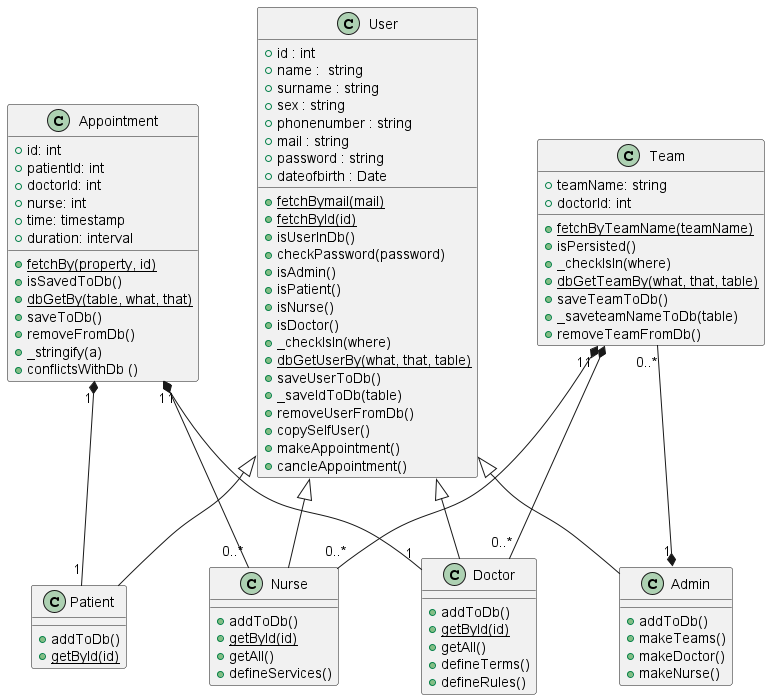
\includegraphics[width=\textwidth]{slike/backend_class_diagram.png} %veličina u odnosu na širinu linije
			            \caption{Dijagram razreda - Modeli}
			            \label{fig:class1} %label mora biti drugaciji za svaku sliku
		      \end{figure}
		      
		      \eject
		      
		      
		        Dijagram razreda na slici 4.5 generirali smo pomoću 'Classdiagram -ts' ekstenzije autora Alexa Shena u razvojnom okruženju Visual Studio Code. Dijagram prikazuje strukturu frontend dijela aplikacije. Angular je framework koji se bazira na komponentama, te svaka komponenta, koja je osnovni i gradivni dio, koristi neki od modula koji ih povezuju. Tako korijenski modul aplikacije, AppRoutingModule koristi svi nadređene module kao što su HomeModule, TeamModule, AdminModule, PatientModule, TechModule i DoctorModule, a svaka od njih koriste MainFooterModule i MainNavigationModule. Korištenjem komponenata smanjujemo redundanciju u kodu. Ovisno o tome koje ovlasti ima, bio on doktor, medicinska sestra pacijent ili administator, korisniku su prikazane različite komponente. Na primjer, pacijent ima pristup komponentama: KalendarComponent, MainNavigationComponent i MainFooterComponet.Za svaku komponentu korisniku su prikazani njihovi html predlošci, css oblikovanja i funkcionlanosti definirane u pojedinom dijelu komponente.
                 
		      
		   \begin{figure}[H]
			            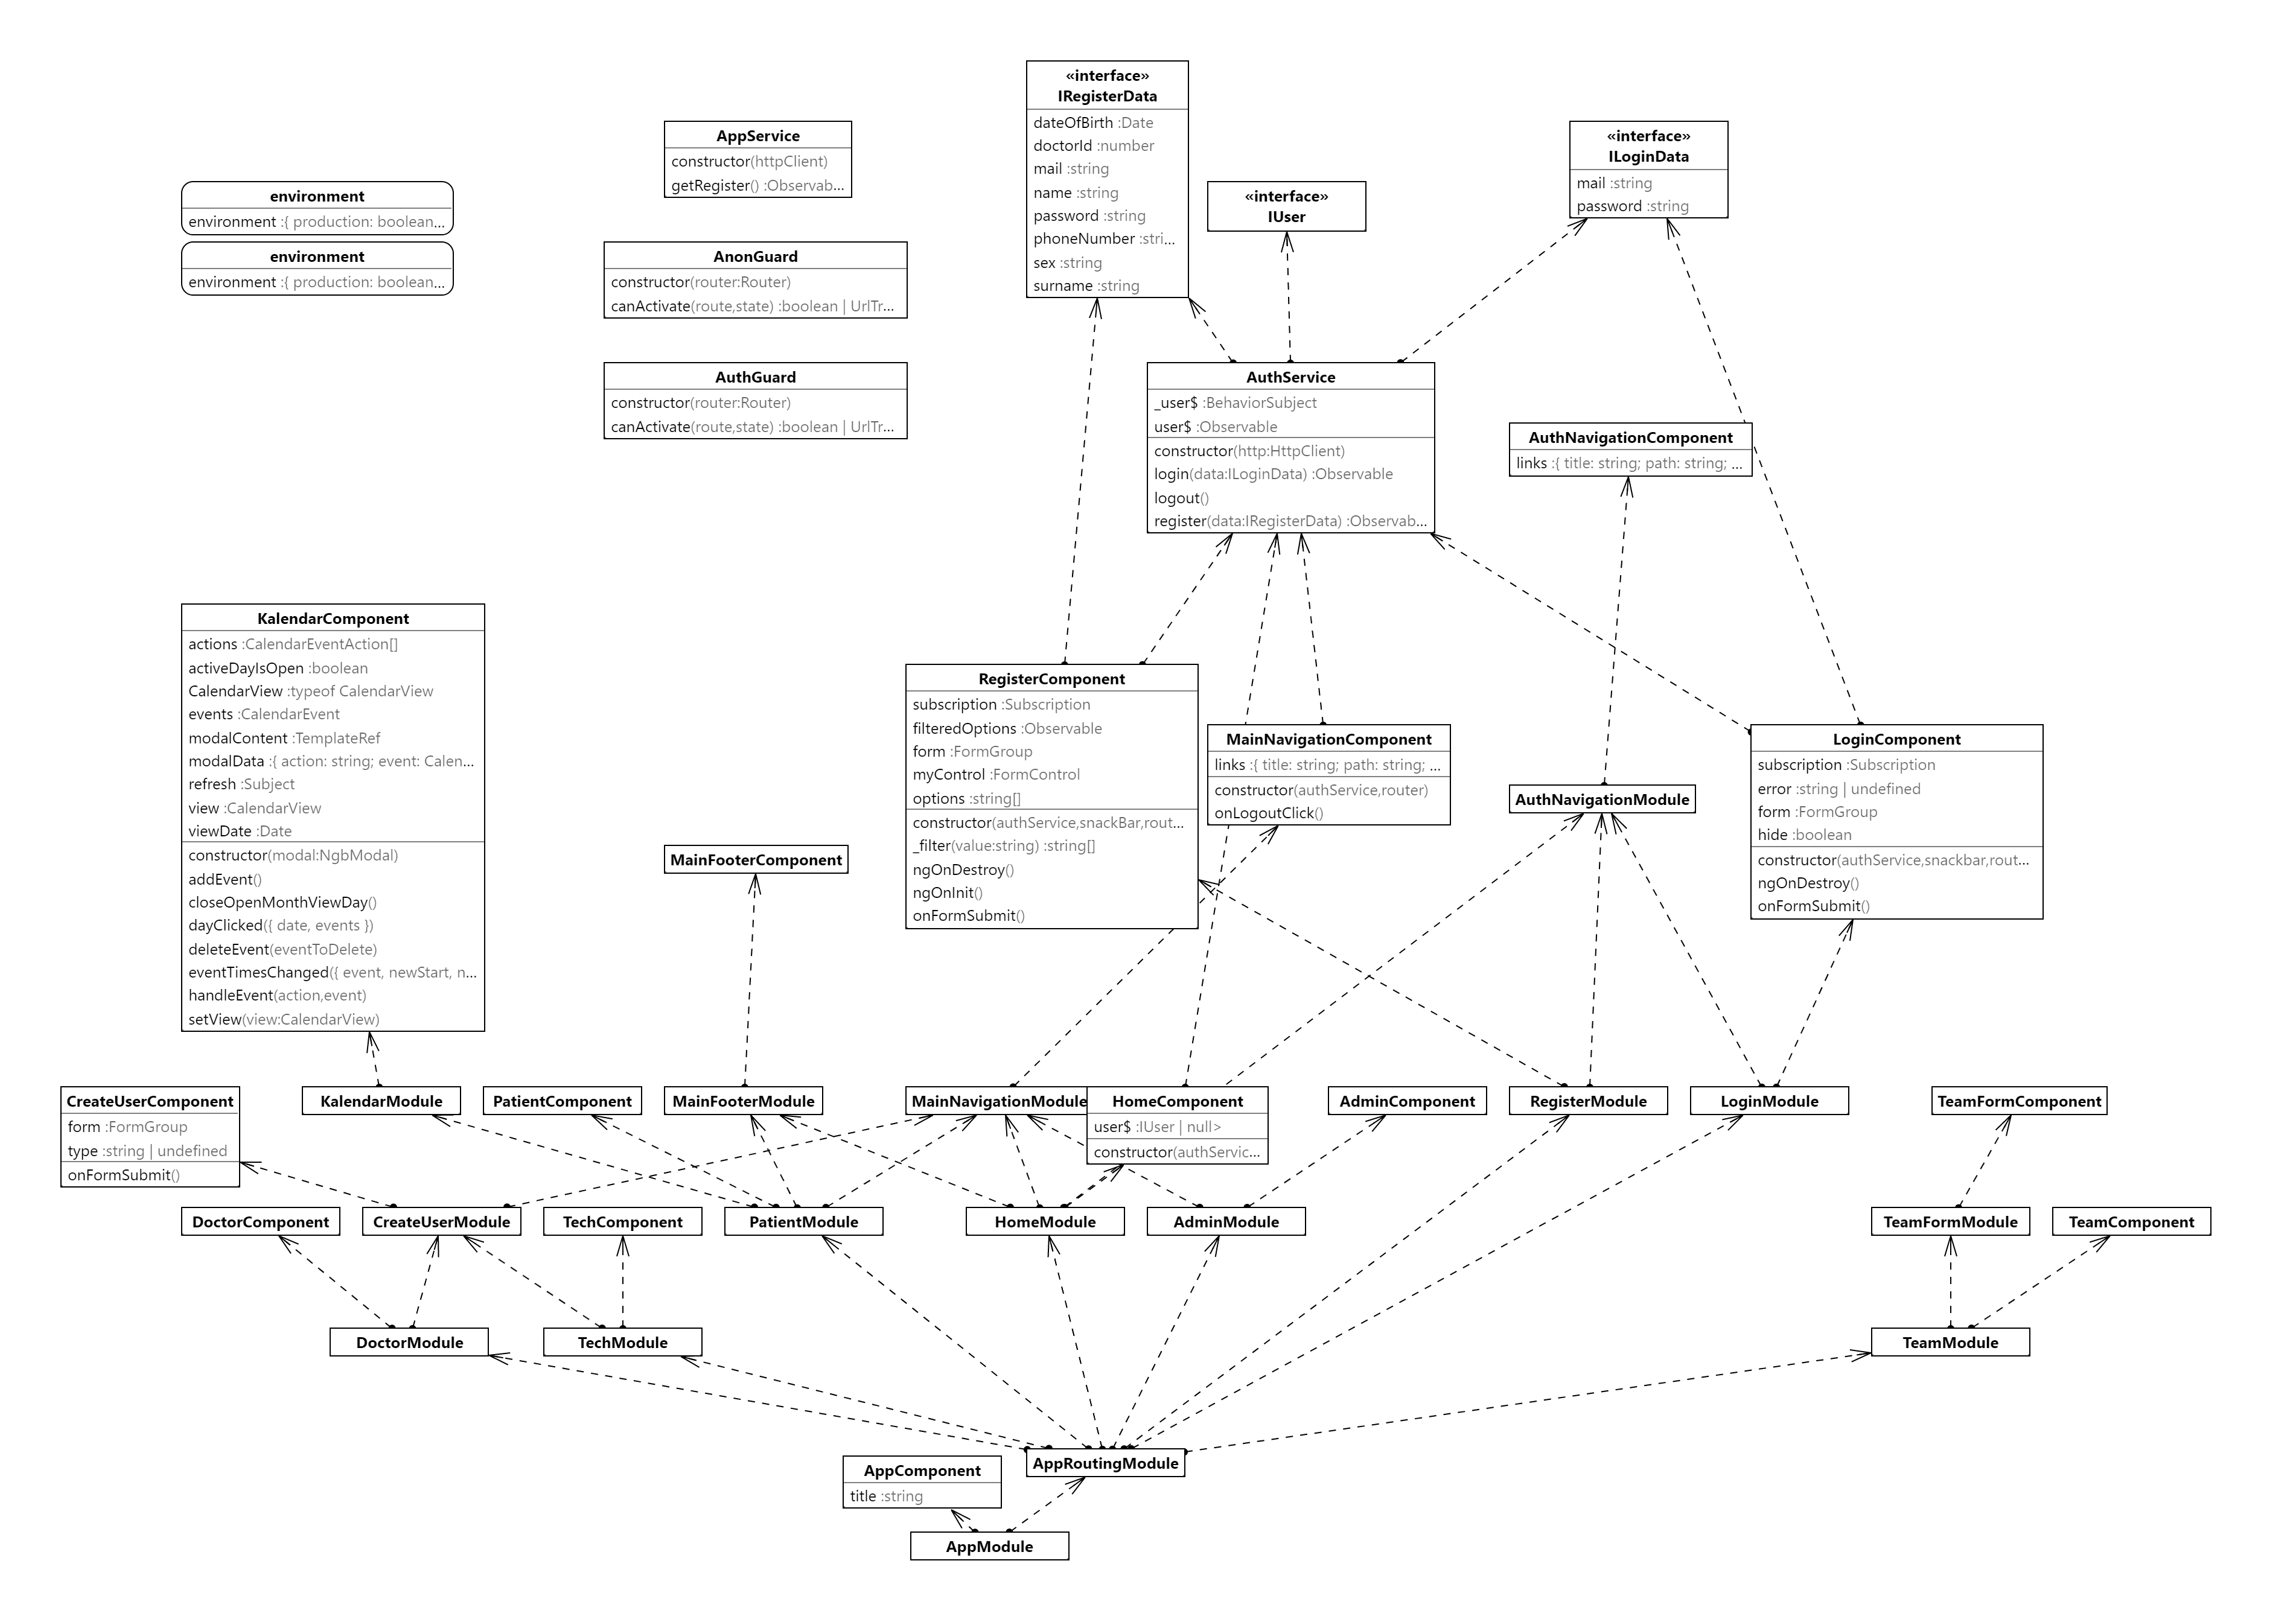
\includegraphics[width=\textwidth]{slike/frontend_class_diagram.png} %veličina u odnosu na širinu linije
			          \caption{Dijagram razreda - frontend}
			            \label{fig:class2} %label mora biti drugaciji za svaku sliku
		      \end{figure}
                 
                
			
		%	\textbf{\textit{dio 2. revizije}}\\			
			
		%\textit{Prilikom druge predaje projekta dijagram razreda i opisi moraju odgovarati stvarnom stanju implementacije}
			
			
			
			\eject
		
		\section{Dijagram stanja}
			
			
			%\textbf{\textit{dio 2. revizije}}\\
			
                      \begin{figure}[H]
			            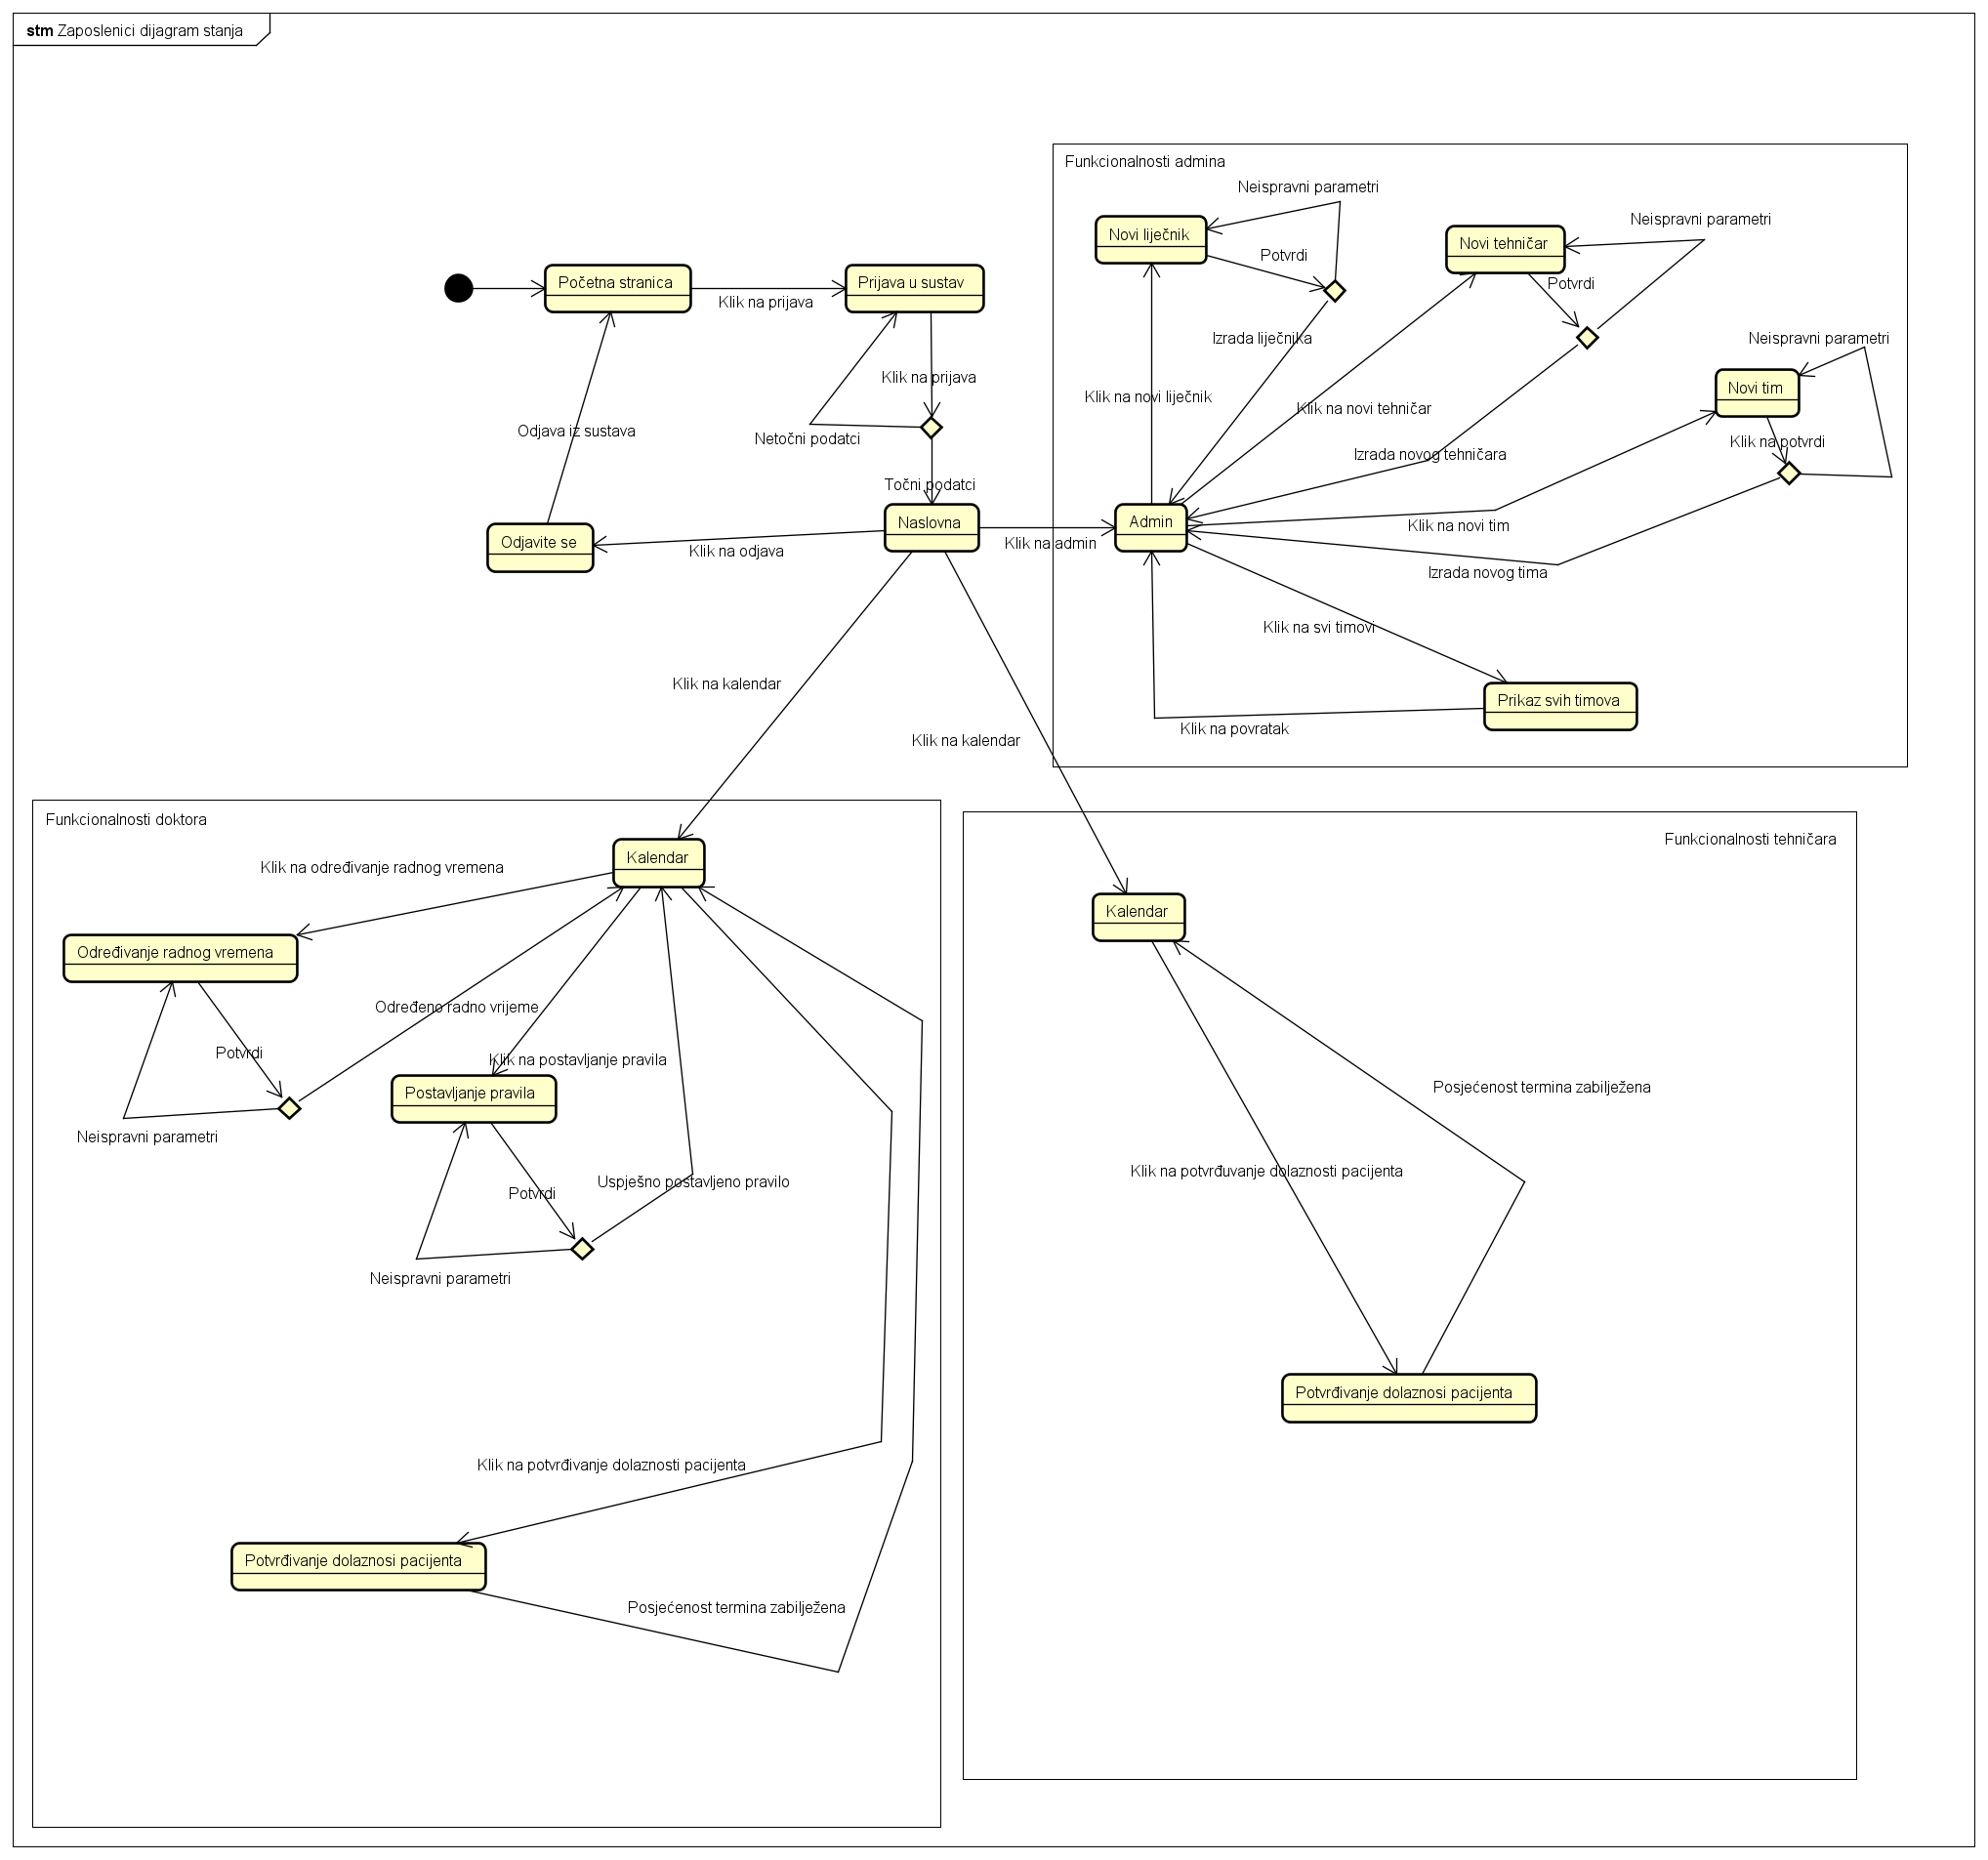
\includegraphics[width=\textwidth]{Zaposlenici.png} %veličina u odnosu na širinu linije
			          \caption{Dijagram stanja zaposlenika}
			            \label{fig:class2} %label mora biti drugaciji za svaku sliku
		      \end{figure}

         \begin{figure}[H]
			            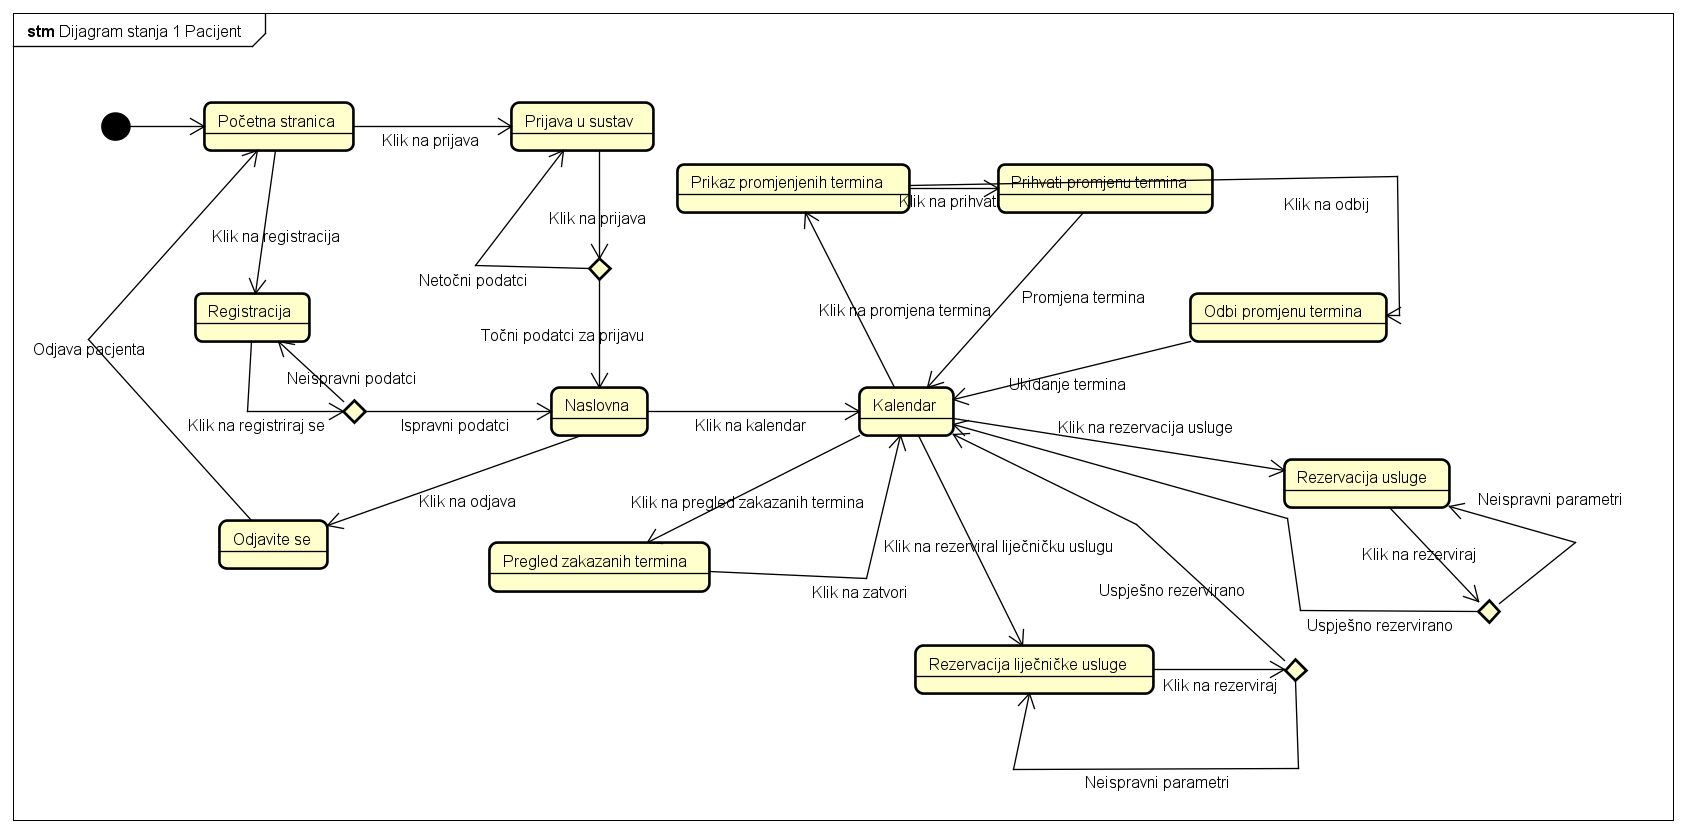
\includegraphics[width=\textwidth]{Dijagram stanja 1 Pacijent.png} %veličina u odnosu na širinu linije
			          \caption{Dijagram stanja pacijenta}
			            \label{fig:class2} %label mora biti drugaciji za svaku sliku
		      \end{figure}
			
			
			\eject 
		\section{Dijagram aktivnosti}
  
			 \begin{figure}[H]         %DODAO SAM TU BROJ 0.88
			            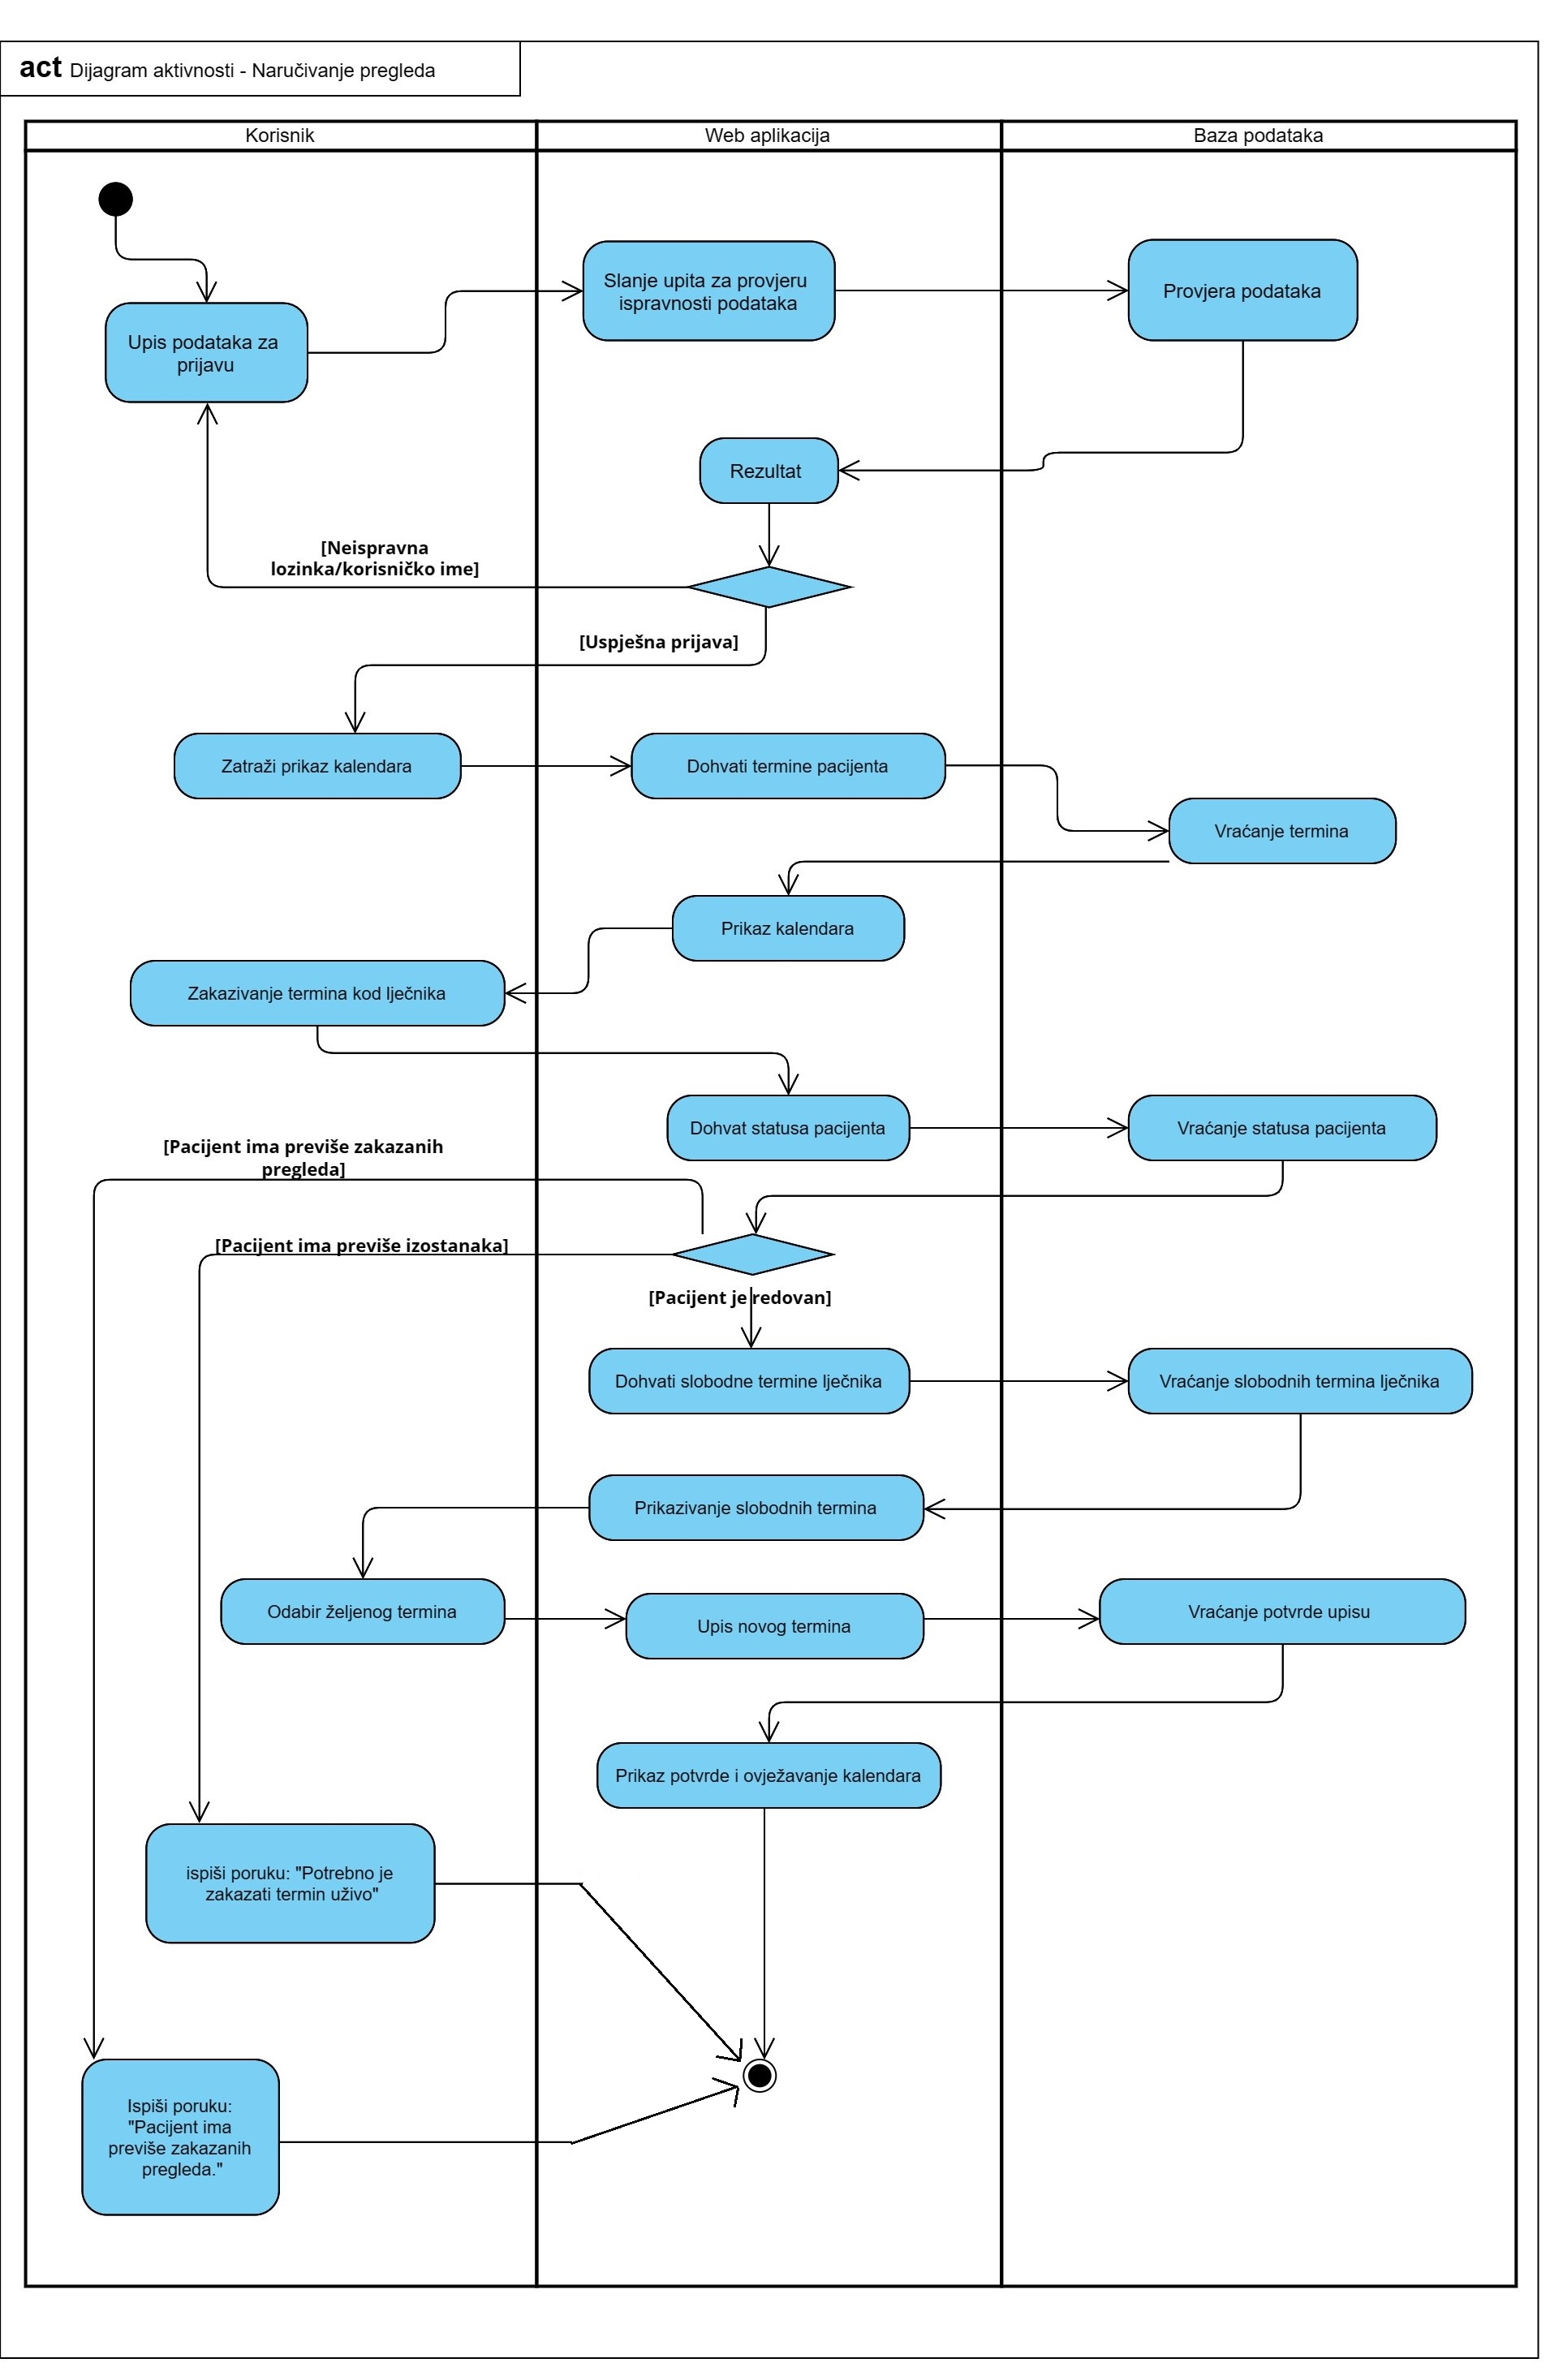
\includegraphics[width=0.88\textwidth]  {slike/dijagram_aktivnosti_v2.jpg} %veličina u odnosu na širinu linije
			          \caption{Dijagram aktivnosti}
			            \label{fig:act} %label mora biti drugaciji za svaku sliku
		      \end{figure}
                 \texttt{}{
                 Na slici 4.8. prikazan je dijagram aktivnosti sustava za naručivanje. Opisan je slučaj naručivanja pregleda. Iako je u dijagramu detaljno opisana radnja naručivanja, ovdje ćemo je sažeti. Korisnik se prijavljuje u sustav, ukoliko je unio pogrešne podatke sustav ga vraća na početak. Ukoliko su podatci postojani, tada se prikazuje kalendar korisniku. Nakon toga aplikacija ispituje je li status pacijenta redovan. Ako je, pacijentu se dozvoljava odabir termina. Ako je pacijent imao previše izostanaka, šalje ga da zakaže sastanak s doktorom uživo. Ako je pacijent imao previše zakazanih pregleda, ispisuje se poruka: "Pacijent ima previše zakazanih pregleda".
                 }
			
			\eject
		\section{Dijagram komponenti}
		
			%\textbf{\textit{dio 2. revizije}}\\
		
			 %\textit{Potrebno je priložiti dijagram komponenti s pripadajućim opisom. Dijagram komponenti treba prikazivati strukturu cijele aplikacije.}
			 
			 Na slici 4.9 prikazan je dijagram komponenti. Korisnik iz web preglednika pristupa aplikaciji korištenjem REST API-ja. Sama aplikacija se sastoji od dvije komponente. Prva komponenta odgovara frontendu i izgrđena je korištenjem Angular biblioteke. Druga komponenta odgovara backendu i izgradena je korištenjem radnog okvira Express. Frontend i backend komuniciraju korištenjem REST API-ja. Baza podataka je relacijska i backend joj pristupa slanjem SQL upita.
			 
			 \begin{figure}[H]
			            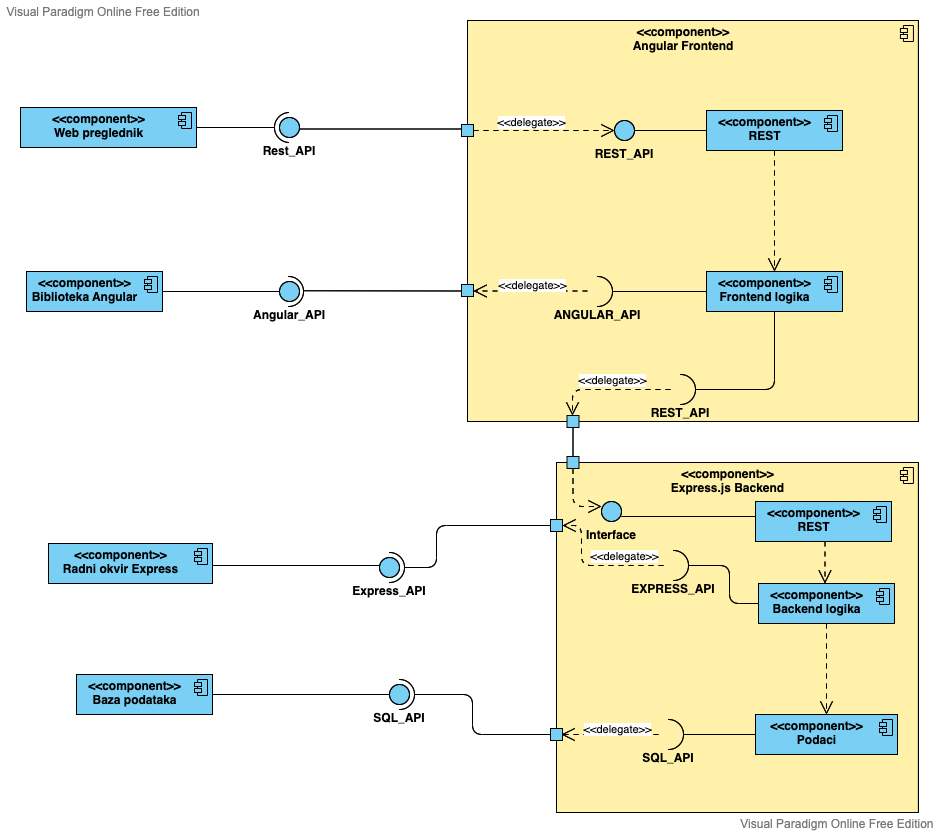
\includegraphics[width=\textwidth]{slike/komponenti_v2.png} %veličina u odnosu na širinu linije
			          \caption{Dijagram komponenti}
			            \label{fig:comp} %label mora biti drugaciji za svaku sliku
		      \end{figure}